% !TEX TS-program = pdflatex
% !TEX encoding = UTF-8 Unicode

% This is a simple template for a LaTeX document using the "article" class.
% See "book", "report", "letter" for other types of document.

\documentclass[11pt]{article} % use larger type; default would be 10pt

\usepackage[utf8]{inputenc} % set input encoding (not needed with XeLaTeX)

%%% Examples of Article customizations
% These packages are optional, depending whether you want the features they provide.
% See the LaTeX Companion or other references for full information.

%%% PAGE DIMENSIONS
\usepackage{geometry} % to change the page dimensions
\geometry{a4paper} % or letterpaper (US) or a5paper or....
% \geometry{margin=2in} % for example, change the margins to 2 inches all round
% \geometry{landscape} % set up the page for landscape
%   read geometry.pdf for detailed page layout information

\usepackage{graphicx} % support the \includegraphics command and options

% \usepackage[parfill]{parskip} % Activate to begin paragraphs with an empty line rather than an indent

%%% PACKAGES
\usepackage{booktabs} % for much better looking tables
\usepackage{array} % for better arrays (eg matrices) in maths
\usepackage{paralist} % very flexible & customisable lists (eg. enumerate/itemize, etc.)
\usepackage{verbatim} % adds environment for commenting out blocks of text & for better verbatim
\usepackage{subfig} % make it possible to include more than one captioned figure/table in a single float
\usepackage{graphicx}
% These packages are all incorporated in the memoir class to one degree or another...

%%% HEADERS & FOOTERS
\usepackage{fancyhdr} % This should be set AFTER setting up the page geometry
\pagestyle{fancy} % options: empty , plain , fancy
\renewcommand{\headrulewidth}{0pt} % customise the layout...
\lhead{}\chead{}\rhead{}
\lfoot{}\cfoot{\thepage}\rfoot{}

%%% SECTION TITLE APPEARANCE
\usepackage{sectsty}
\allsectionsfont{\sffamily\mdseries\upshape} % (See the fntguide.pdf for font help)
% (This matches ConTeXt defaults)

%%% ToC (table of contents) APPEARANCE
\usepackage[nottoc,notlof,notlot]{tocbibind} % Put the bibliography in the ToC
\usepackage[titles,subfigure]{tocloft} % Alter the style of the Table of Contents
\renewcommand{\cftsecfont}{\rmfamily\mdseries\upshape}

%%% END Article customizations

%%% The "real" document content comes below...

\title{Documetaci\'on Base de datos}
\author{David G\'omez S\'anchez y Pablo Vicente Munuera}
\date{} % Activate to display a given date or no date (if empty),
         % otherwise the current date is printed 

\begin{document}
\maketitle

\begin{abstract}

Esto es un abstract. Y como tal, proceder\'a a relatarle, un esbozo de lo que es este documento. En él, trataremos temas tan acuciantes como: ?`Qu\'e es esto? ?`C\'omo hemos trabajado? ?`Qu\'e problemas hemos sobrepasado? y ?`C\'omo se ejecuta nuestro \emph{wonderful} programa?

\end{abstract}

\section{Introducci\'on}

Your text goes here.

\section{Getting started}

Aunque est\'a explicado como preparar el entorno para ejecutar nuestros programas, procederemos a hacerlo, igualmente, aqu\'i.

\begin{figure}
\centering
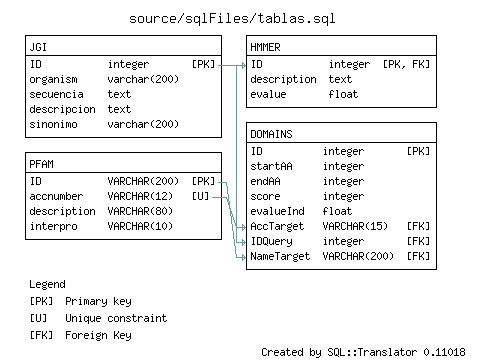
\includegraphics[width=15cm]{design}
\caption{Dise\~no final de la base de datos\label{fig:Design}}
\end{figure}

\section{Realizaci\'on de la pr\'actica}

\subsection{Dise\~no de base de datos}

El dise\~no de base de datos nos ha llevado de cabeza durante la mayor parte del desarrollo del trabajo, aunque eso trataremos m\'as debidamente en la secci\'on: problemas encontrados.

Ha habido dos tablas claras desde el primero momento: la tabla jgi y la tabla Pfam. La primera representa al punto 1.a ''Procedente de jgi'' y corresponde a las prote\'inas y sus correspondientes secuencias y datos. Tiene como clave primaria el id, lo cual parece l\'ogico, ya que es el elemento m\'as representativo de cada prote\'ina. Aunque en un primer momento se puso tambi\'en el organismo, posteriormente se vi\'o que el id cambiaba con el organismo, con lo que no era necesaria la dupla id-organismo como clave primaria. Por otro lado, la tabla Pfam tambi\'en qued\'o bastante resuelta desde un principio. A parte de los datos que se nos informaba que deb\'ia contener esta tabla, lo \'unico que hab\'ia que pensar era la clave primaria y la posibilidad de claves alternativas. Las dos \'unicas cosas que no se pueden repetir es el ID y el accesion number. La combinaci\'on de ambas no era posible, ya que no para un mismo ID no va a haber 2 accesion number distintos, ser\'a siempre el mismo, con lo que se opta por poner una clave primaria (ID, pero podr\'ia haber sido perfectamente el accesion number) y una clave alternativa que ser\'a el accesion number.  Un dato curioso: intentando imitar lo que se di\'o en clase, se hizo una tabla para los accesion number y los posibles accesion numbers antiguos. Esta se acab\'o por eliminar, ya que no ten\'ia mucho sentido en el entorno de la pr\'actica.

 El problema y la parte de las tablas que m\'as cambios han sufrido ha sido la tabla correspondiente al punto 1.c ''Datos provenientes de hmmer''. Ha llegado a haber hasta 3 tablas, s\'olo para esta secci\'on.



\subsection{Problemas encontrados}

\section{Conclusi\'on}



\end{document}
